	\tikzset{%
			every neuron/.style={
				circle,
				draw,
				minimum size=1cm
			},
			neuron missing/.style={
				draw=none, 
				%scale=4,
				%rotate=90,
				%yshift=1,
				%text height=0.333cm,
				%execute at begin node=\color{black}$\cdots$
			},
		}
		\begin{figure}[H]
			\centering
				
				
				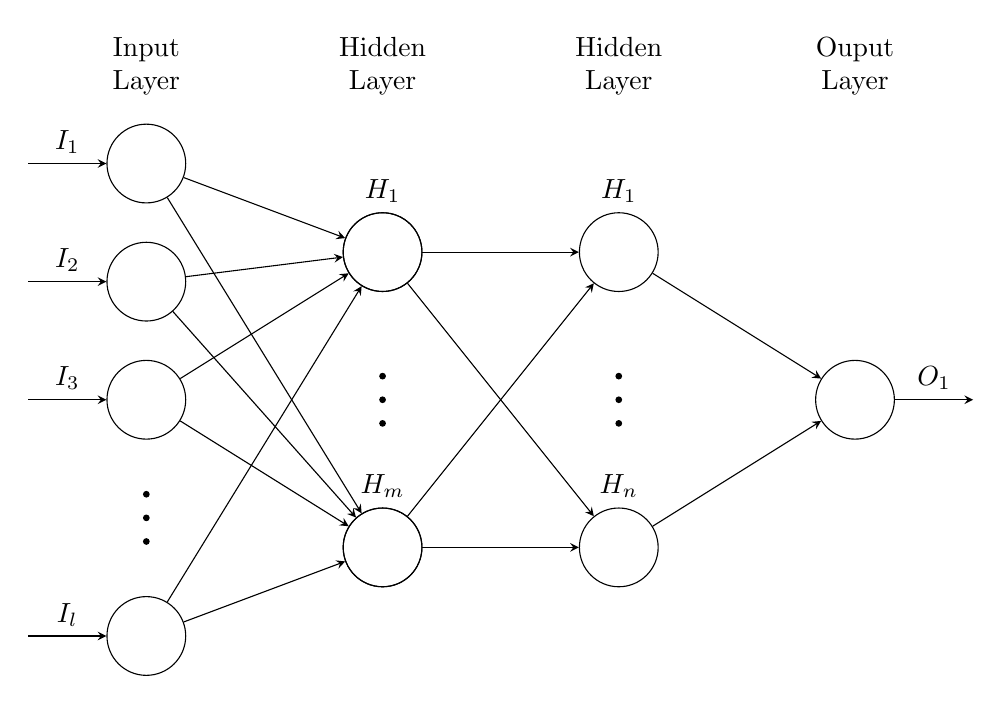
\begin{tikzpicture}[x=1.5cm, y=1.5cm, >=stealth]
					
					\foreach \m/\l [count=\y] in {1,2,3,missing,4}
					\node [every neuron/.try, neuron \m/.try] (input-\m) at (0,2.5-\y) {};
					
					\foreach \m [count=\y] in {1,missing,2}
					\node [every neuron/.try, neuron \m/.try ] (hidden1-\m) at (2,2-\y*1.25) {};
					
					\foreach \m [count=\y] in {1,missing,2}
					\node [every neuron/.try, neuron \m/.try ] (hidden1-\m) at (2,2-\y*1.25) {};
					
					\foreach \m [count=\y] in {1,missing,2}
					\node [every neuron/.try, neuron \m/.try ] (hidden2-\m) at (4,2-\y*1.25) {};
					
					\foreach \m [count=\y] in {1}
					\node [every neuron/.try, neuron \m/.try ] (output-\m) at (6,0.5-\y) {};
					
					\foreach \l [count=\i] in {1,2,3,l}
					\draw [<-] (input-\i) -- ++(-1,0)
					node [above, midway] {$I_\l$};
					
					\foreach \l [count=\i] in {1,m}
					\node [above] at (hidden1-\i.north) {$H_\l$};
					
					\foreach \l [count=\i] in {1,n}
					\node [above] at (hidden2-\i.north) {$H_\l$};
					
					\foreach \l [count=\i] in {1}
					\draw [->] (output-\i) -- ++(1,0)
					node [above, midway] {$O_\l$};
					
					\foreach \i in {1,...,4}
					\foreach \j in {1,...,2}
					\draw [->] (input-\i) -- (hidden1-\j);
					
					\foreach \i in {1,...,2}
					\foreach \j in {1,...,2}
					\draw [->] (hidden1-\i) -- (hidden2-\j);
					
					\foreach \i in {1,...,2}
					\foreach \j in {1}
					\draw [->] (hidden2-\i) -- (output-\j);
					
					\foreach \l [count=\x from 0] in {Input, Hidden, Hidden, Ouput}
					\node [align=center, above] at (\x*2,2) {\l \\ Layer};
					\draw[fill=black](0,-1.3)circle(1pt);
					\draw[fill=black](0,-1.5)circle(1pt);
					\draw[fill=black](0,-1.7)circle(1pt);
					\draw[fill=black](2,-0.3)circle(1pt);
					\draw[fill=black](2,-0.5)circle(1pt);
					\draw[fill=black](2,-0.7)circle(1pt);
					\draw[fill=black](4,-0.3)circle(1pt);
					\draw[fill=black](4,-0.5)circle(1pt);
					\draw[fill=black](4,-0.7)circle(1pt);
					
				\end{tikzpicture}
		
		\caption{Darstellung des entwickelten neuronalen Netzes. Neuronen sind hier als Kreise gekennzeichnet. Fortsetzungen sind hier sinngemäß mit drei aufeinander folgenden Punkten dargestellt. Die Besonderheit ist die Reduktion der Ausgabeschicht auf lediglich einen Datenpunkt. Adaptiert aus \cite{neuron}}
		\label{fig: ownnet}
		\end{figure}